\section{Conventional Boost Converter}\label{ch:CBC}
\todo[color=c04a,inline]{Conventional Boost Converter}

\subsection{Principle of operation}\label{sec:CBC_POC}

The conventional boost converter uses one inductor,
one switch and one capacitor. When the switch is closed, the inductor current rises and energy is stored in the inductor L. When the switch is open, the inductor discharges through diode D and the inductor current falls. It steps up the voltage when
the switch is in OFF state. The two modes of operation will be discussed in this chapter. The circuit can be observed on figure..


\begin{figure}[H]
   \centering
   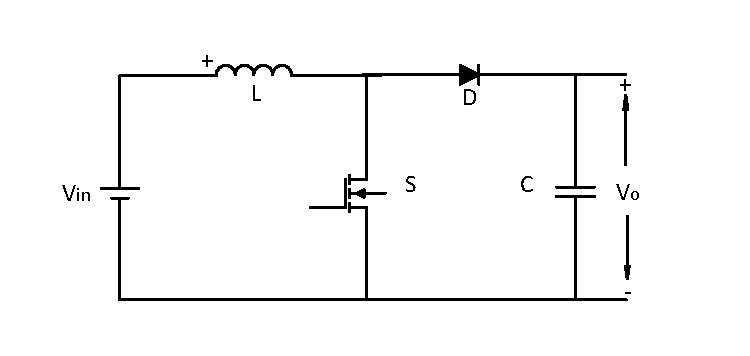
\includegraphics[width=\textwidth]{figures/aConventionalBoost/ConventionalBoostConverter.pdf}
    \caption{Conventional Boost Converter}
	\label{fig:ConventionalBoost}
\end{figure}

\subsection{Operation Modes}\label{sec:CBC_OP}

Switch ON:

When the switch is ON,
the inductor is being charged and the capacitor discharges over the load resistor.

\begin{figure}[H]
   \centering
   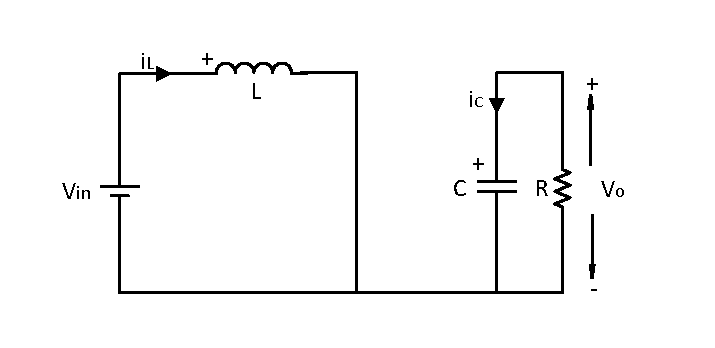
\includegraphics[width=\textwidth]{figures/aConventionalBoost/ConventionalBoostConverterON.pdf}
    \caption{Conventional Boost Converter Switch ON}
	\label{fig:ConventionalBoostON}
\end{figure}

In this case we have:
\begin{equation}
	V_L = V_{in}
	\label{eq:CBC_SWON1}
\end{equation}
where
\begin{equation}
	V_L = L \frac{di}{dt}
	\label{eq:CBC_SWON2}
\end{equation}
and
\begin{equation}
	V_C = V_R
	\label{eq:CBC_SWON3}
\end{equation}
The capacitor current discharges over the resistor:
\begin{equation}
	i_C = -\frac{V_o}{R}
	\label{eq:CBC_SWON4}
\end{equation}


Switch OFF:

\begin{figure}[H]
   \centering
   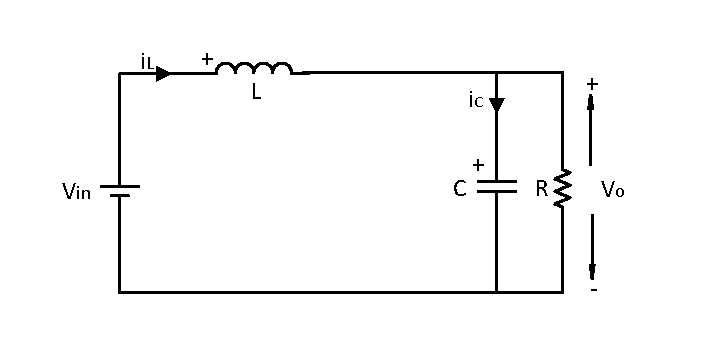
\includegraphics[width=\textwidth]{figures/aConventionalBoost/ConventionalBoostConverterOFF.pdf}
    \caption{Conventional Boost Converter Switch OFF}
	\label{fig:ConventionalBoostOFF}
\end{figure}

When the switch is OFF,
the capacitor is being charged and this is the mode when the boosting happens.

In this case we have:
\begin{equation}
	V_L = V_{in} - V_o
	\label{eq:CBC_SWOFF1}
\end{equation}

\begin{equation}
	i_C = i_L -\frac{V_o}{R}
	\label{eq:CBC_SWOFF2}
\end{equation}

\begin{figure}[H]
   \centering
   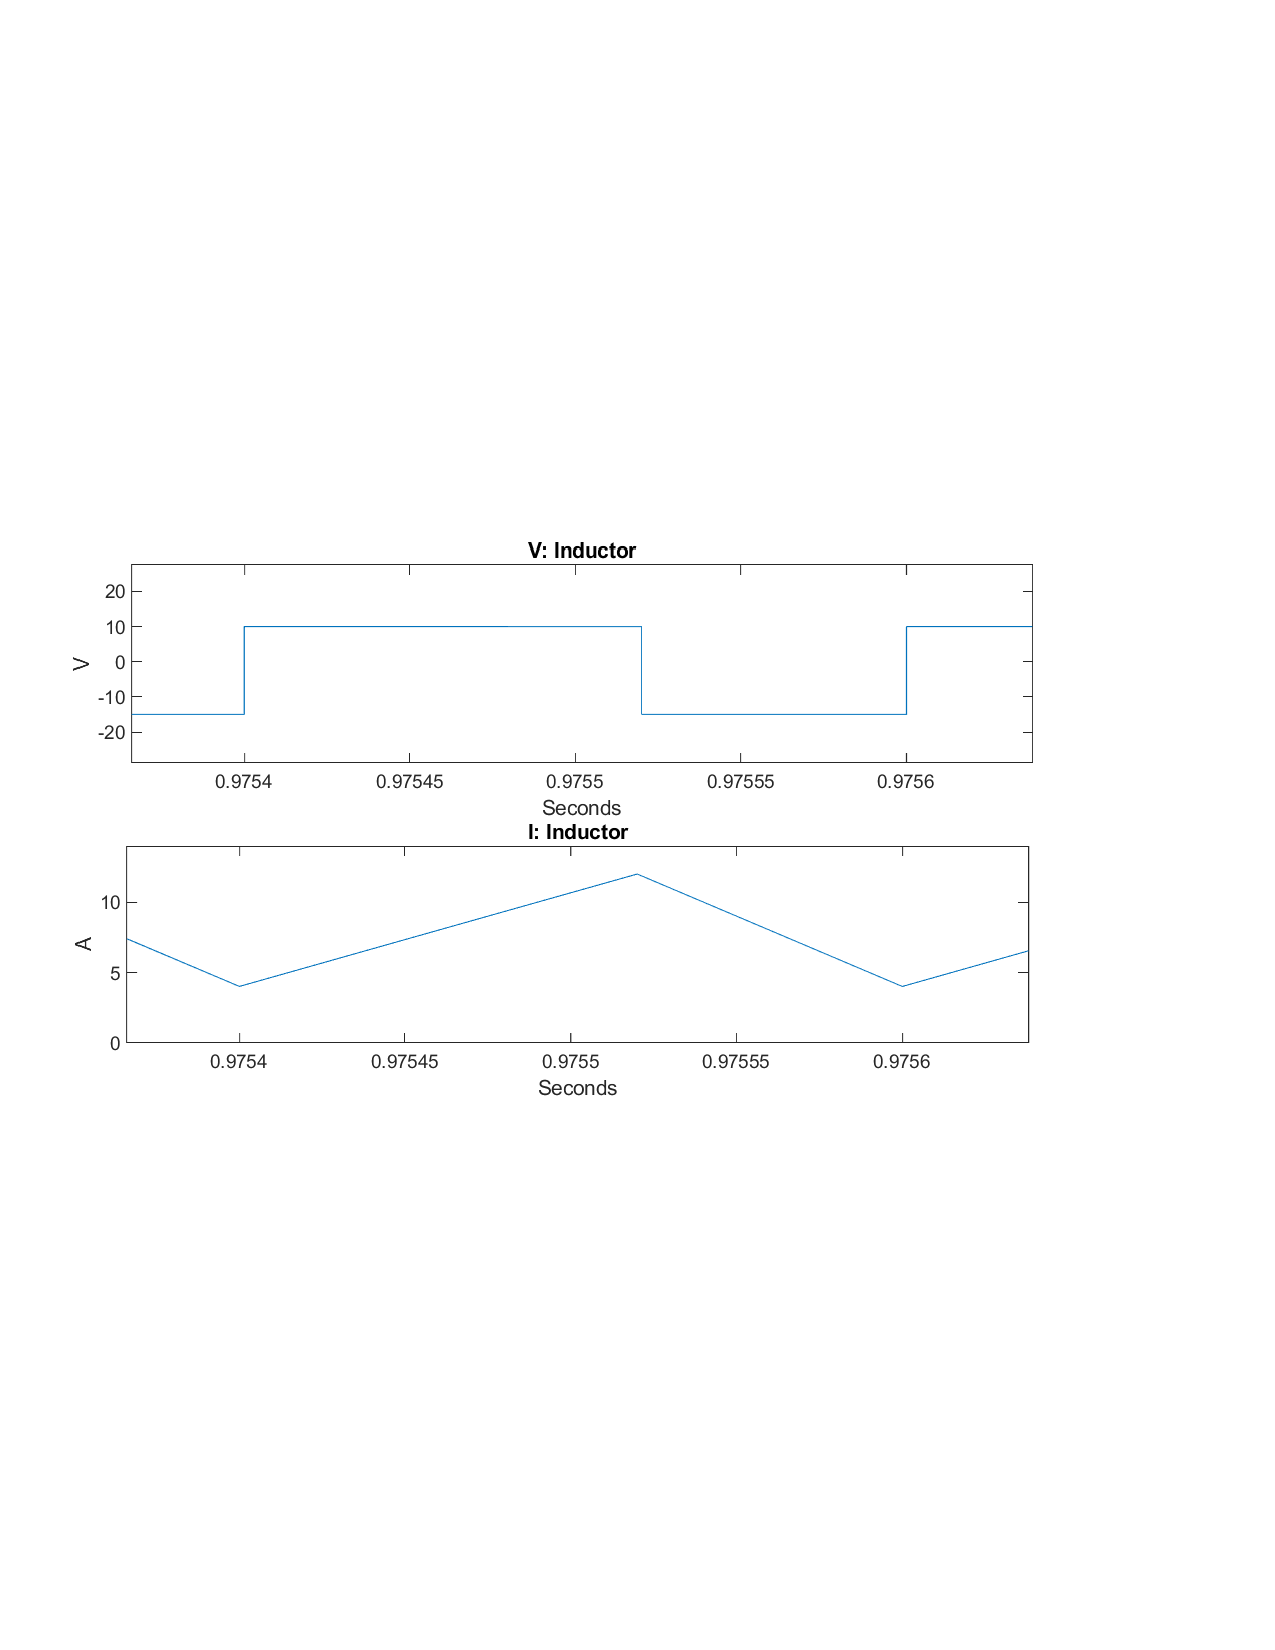
\includegraphics[width=\textwidth]{figures/aConventionalBoost/LvAndLi.pdf}
    \caption{CBC Inductor Wave Forms}
	\label{fig:ConventionalBoostOFF}
\end{figure}

\subsection{Convertion ratio}\label{sec:convertionRatio}

Based on inductor volt-second balance, the convertion ratio can be calculated:

\begin{equation}
	\int_{0}^{T_s} v_L(t)dt = V_{in}D + (V_{in}-V_{out})(1-D) = 0
	\label{eq:CBC_VISB}
\end{equation}

\begin{equation}
	\frac{V_o}{V_{in}} = \frac{1}{1-D}
	\label{eq:CBC_CR}
\end{equation}

\subsection{Inductor current ripple}\label{sec:CBC_ICR}

The inductor current slope for the interval from 0 to DTs can be found as:

\begin{figure}[H]
   \centering
   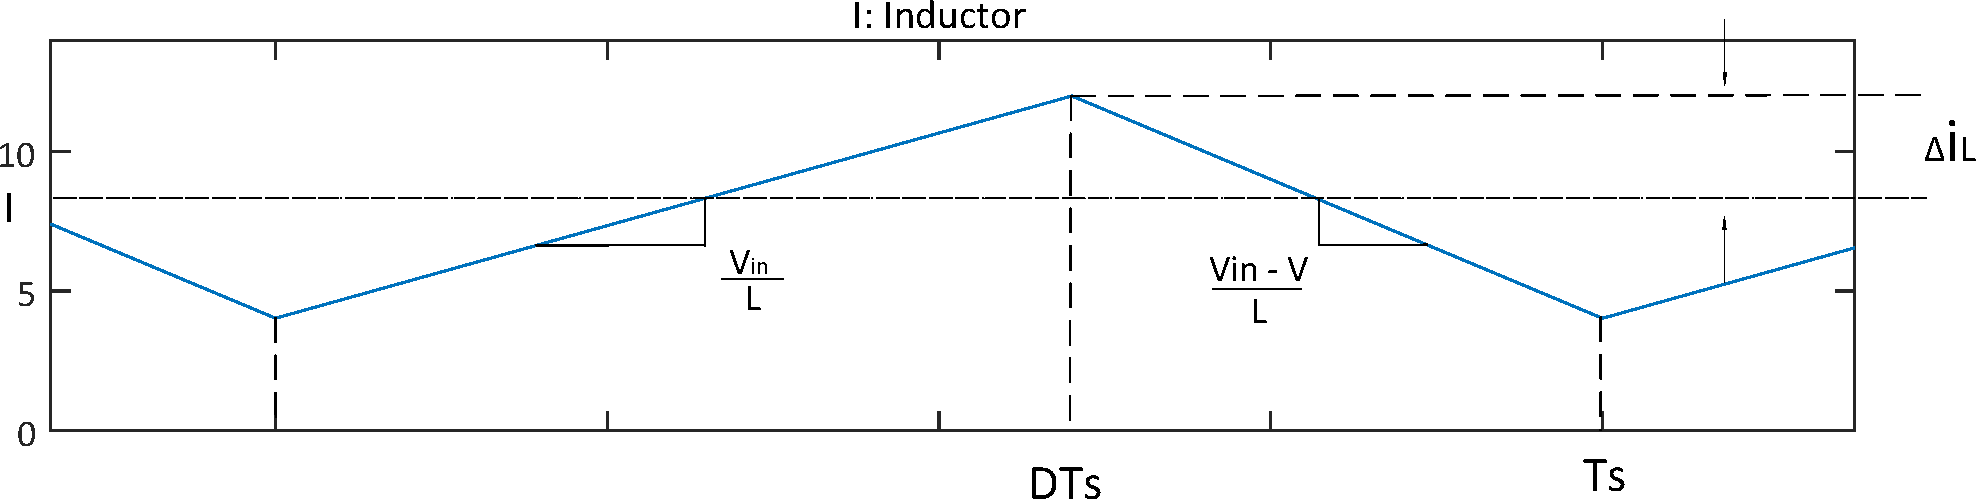
\includegraphics[width=\textwidth]{figures/aConventionalBoost/InductorCurrent.pdf}
    \caption{CBC Inductor Current Ripple}
	\label{fig:InductorCurrent}
\end{figure}


\begin{equation}
	\frac{di_L(t)}{dt} = \frac{v_L(t)}{L} = \frac{V_{in}}{L}
	\label{eq:CBC_ICR1}
\end{equation}

and the current slope for the interval (1 - DTs):

\begin{equation}
	\frac{di_L(t)}{dt} = \frac{v_L(t)}{L} = \frac{V_{in} - V}{L}
	\label{eq:CBC_ICR2}
\end{equation}

The change of inductor current during the first subinterval is:

\begin{equation}
	2\Delta i_L = \frac{V_{in}}{L}DT_s \Rightarrow
  \Delta i_L = \frac{V_{in}}{2L}DT_s
	\label{eq:CBC_ICR3}
\end{equation}

The inductor should be chosen such that a desired ripple magnitude is optained.

\subsection{Capacitor voltage ripple}\label{sec:CBC_CVR}

\begin{figure}[H]
   \centering
   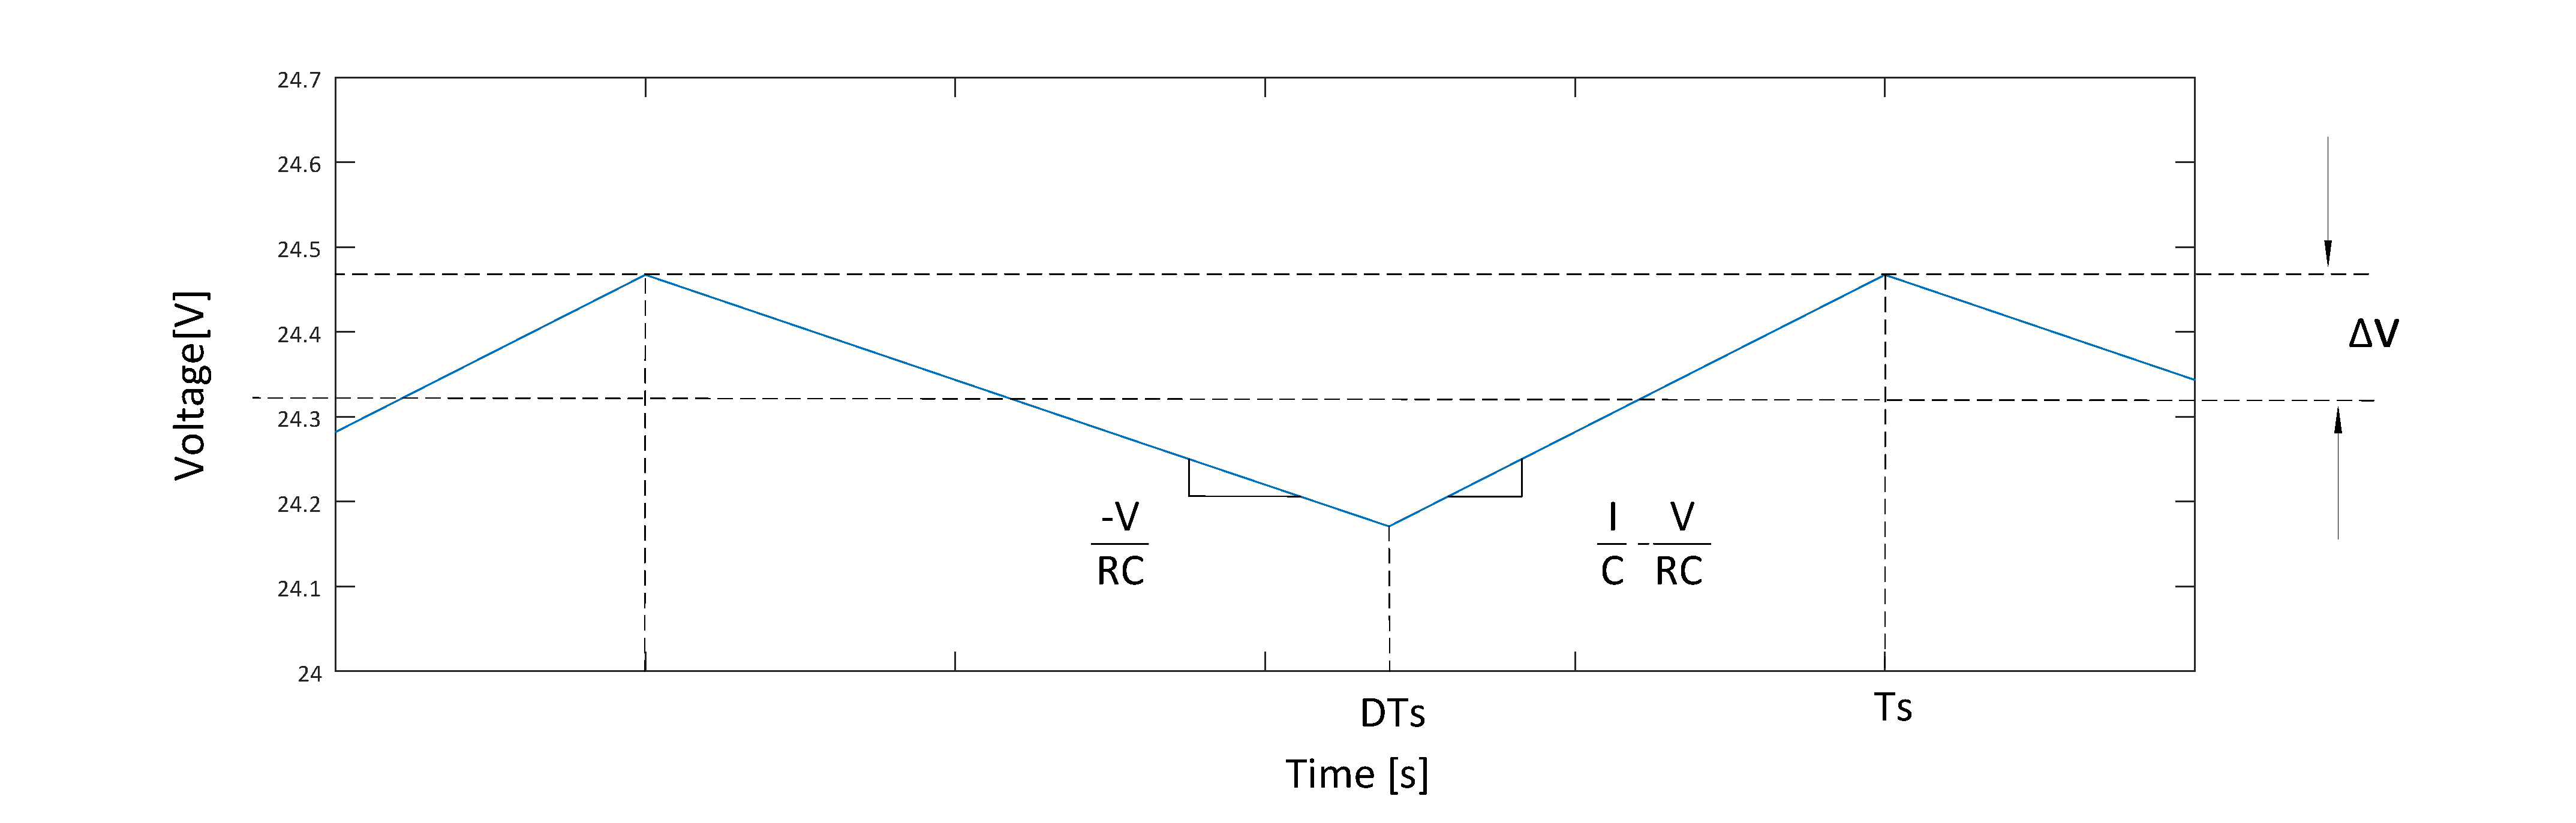
\includegraphics[width=\textwidth]{figures/aConventionalBoost/CapacitorVoltage.pdf}
    \caption{Capacitor Voltage Ripple}
	\label{fig:CBC_CVR1}
\end{figure}

The capacitor voltage slope for the interval from 0 to DTs can be found as:

\begin{equation}
	\frac{dv_c(t)}{dt} = \frac{i_c(t)}{C} = \frac{-V}{RC}
	\label{eq:CBC_CVR2}
\end{equation}

and the voltage slope for the interval (1 - DTs):

\begin{equation}
	\frac{dv_c(t)}{dt} = \frac{i_c(t)}{C} = \frac{I}{C} - \frac{V}{RC}
	\label{eq:CBC_CVR3}
\end{equation}

The change of capacitor voltage during the first subinterval is:

\begin{equation}
	-2\Delta v = \frac{-V}{RC}DT_s \Rightarrow
  \Delta v = \frac{V}{2RC}DT_s
	\label{eq:CBC_CVR4}
\end{equation}

The capacitor should be chosen according to the desired voltage ripple.

\subsection{Design Example}\label{sec:CBC_DE}

If we consider a design for a boost converter that will have an output of 25V from a 10V source, with a continuous inductor current and an output voltage of less than one percent, we will have the following parameters:


V\textsubscript{in} = 10 V, V\textsubscript{out} = 25 V and D = 0.6. Also,
a load resistor of 40 $\Omega$ and a  switching frequency of 25kHz are considered for the design.

By the fact that the average power supplied by the source must be the same as the average power absorbed by the load resistor, the output power can be obtained by:

\begin{equation}
	P_o = \frac{V^2_o}{R} = V_oI_o
	\label{eq:CBC_CVR4}
\end{equation}

and the input power is $V_{in}I_s = V_{in}I_L$

\begin{equation}
	\Rightarrow V_{in}I_L = \frac{V^2_o}{R} = \frac{[V_{in}/(1-D)]^2}{R}
	\label{eq:CBC_CVR4}
\end{equation}

solving for I\textsubscript{L}, we get:

\begin{equation}
	I_L = \frac{V_{in}}{(1-D)^2R}
	\label{eq:CBC_CVR4}
\end{equation}

The maximum and minimum inductor current can be determined by:

\begin{equation}
	I_{max} = I_L + \Delta i_L = \frac{V_{in}}{(1-D)^2R} + \frac{V_{in}DT_s}{2L}
	\label{eq:CBC_CVR4}
\end{equation}

\begin{equation}
	I_{min} = I_L - \Delta i_L = \frac{V_{in}}{(1-D)^2R} - \frac{V_{in}DT_s}{2L}
	\label{eq:CBC_CVR4}
\end{equation}

The induction current has to be continuous, so it has to be always positive. This means that I\textsubscript{L} has to be positive and the boundary between continuous and discontinuous inductor current is determined from: 


$I_{min} = 0 = \frac{V_{in}}{(1-D)^2R} - \frac{V_{in}DT_s}{2L}$


or $\frac{V_{in}}{(1-D)^2R} = \frac{V_{in}DT_s}{2L} = \frac{V_{in}D}{2Lf}$


So, the minimum combination of inductance and switching frequency for continuous current is:

\begin{equation}
L_{min} = \frac{D(1-D)^2R}{2f} = \frac{0.6(1-0.6)^2 40}{2\cdot25000} = 76.8\mu F
\end{equation}

L = 100 $\mu$ F to provide a margin to ensure continuous current.
Then, using equations... 

\begin{equation}
I_L = \frac{V_{in}}{(1-D)^2R} = \frac{10}{(1-0.6)^2(40)} = 1.56 A
\end{equation}

Then, from equation...

\begin{equation}
\Delta i_L = \frac{V_{in}DT}{2L} = \frac{10\cdot 0.6}{2\cdot 100\cdot 10^{-6}\cdot 25000} = 1.2 A
\end{equation}

$I_{max} = 1.56 + 1.2 = 2.76 A$ , 
$I_{min} = 1.56 - 1.2 = 0.36 A$

Based on equation.. , the minimum capacitance required to limit the output voltage ripple to 1 percent is:

\begin{equation}
C_{min} = \frac{D}{R\Delta V_of} = \frac{0.6}{40\cdot 0.01\cdot 25000 } = 60\mu F
\end{equation}

